\documentclass{standalone}
\usepackage{tikz}
\usetikzlibrary{matrix,backgrounds,shapes,arrows.meta}

\begin{document}

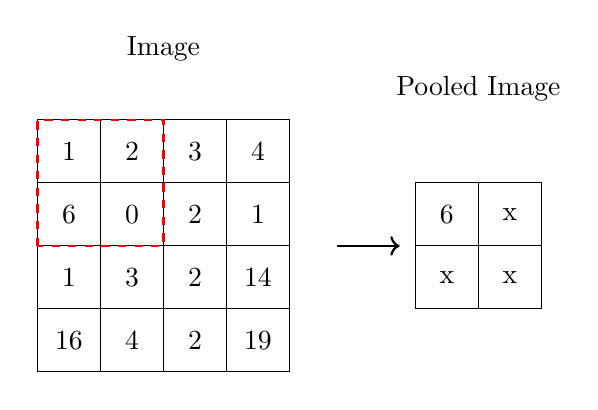
\begin{tikzpicture}

    % Draw the image matrix
    \matrix[matrix of nodes,nodes={draw, minimum size=0.8cm, anchor=center}, column sep=-\pgflinewidth, row sep=-\pgflinewidth] (m) {
        \node {1}; & \node {2}; & \node {3}; & \node {4}; \\
        \node {6}; & \node {0}; & \node {2}; & \node {1}; \\
        \node {1}; & \node {3}; & \node {2}; & \node {14}; \\
        \node {16}; & \node {4}; & \node {2}; & \node {19}; \\
    };

    % Draw a rectangle to indicate the convolution operation area
    \draw[thick, red, dashed] (-1.6,0) rectangle (0,1.6);
    \draw[->, thick] (2.2,0) -- (3,0);


    \matrix[matrix of nodes,nodes={draw, minimum size=0.8cm, anchor=center}, column sep=-\pgflinewidth, row sep=-\pgflinewidth] at (4,0) (b) {
        \node {6}; & \node {x}; \\
        \node {x}; & \node {x}; \\
    };

    % Label the areas
    \node at (0, 2.5) {Image};
    \node at (4, 2) {Pooled Image};


\end{tikzpicture}

\end{document}
